% Graph

\begin{itemize}
    \item \textbf{Node/ Vertex:} Object with name and data (in context of molecules: the atoms)
    \item \textbf{Edge:} Connection between two vertices (in context of molecules: the bond)
    \begin{itemize}
        \item Can be weighted (in context of molecules: single bond and double bond)
        \item Can be directed 
    \end{itemize}
    \item \textbf{Graph:} Collection of nodes and edges
    \begin{center}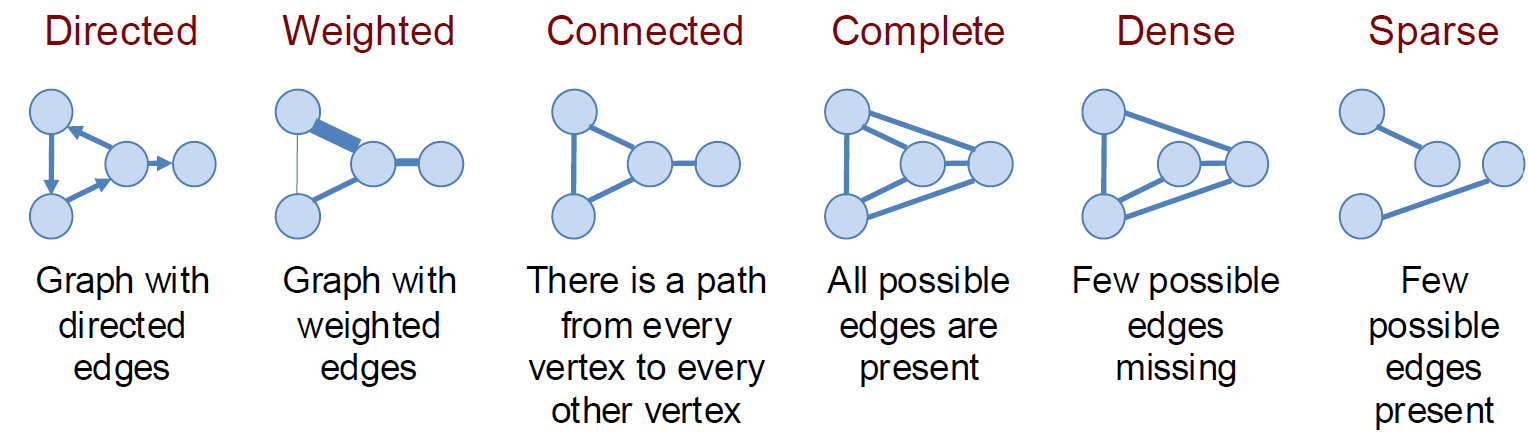
\includegraphics[width=0.85\textwidth]{img/graphs/DifferentGraphs.png}\end{center}
    \item \textbf{Valence of degree of vertex:} Number of edges a vertex lies on (in context of molecules: valence)
    \item \textbf{Adjacent vertices:} Vertices connected by an edge (in context of molecules: neibouring atoms)
    \item \textbf{Path:} List of distinct vertices in which successive vertices are connected by edges
    \begin{itemize}
        \item Simple Path: path with no vertex occurring twice
        \item Cycle Path: simple path of which first and last vertex are the same
    \end{itemize}
    \begin{center}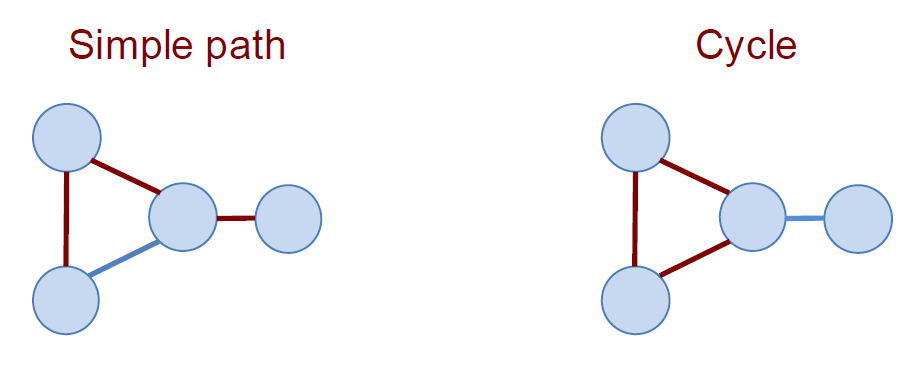
\includegraphics[width=0.85\textwidth]{img/graphs/PathGraphs.png}\end{center}
    \item \textbf{Trees:} (in graph theory)
    \begin{itemize}
        \item \textbf{Tree:} non-empty, acyclic collection of nodes and edges (graph) in which any 2 nodes are connecteds by exactly 1 path.  
        \item \textbf{Ordered Tree:} tree with order in the children nodes
        \item \textbf{Binary Tree:} ordered tree in which each non-terminal node has exactly two children
        \item \textbf{Binary Search Tree:} ordered binary tree with left-to-right order
        \item \textbf{Heap:} ordered binary tree with top-to-bottom order
    \end{itemize}
    \begin{center}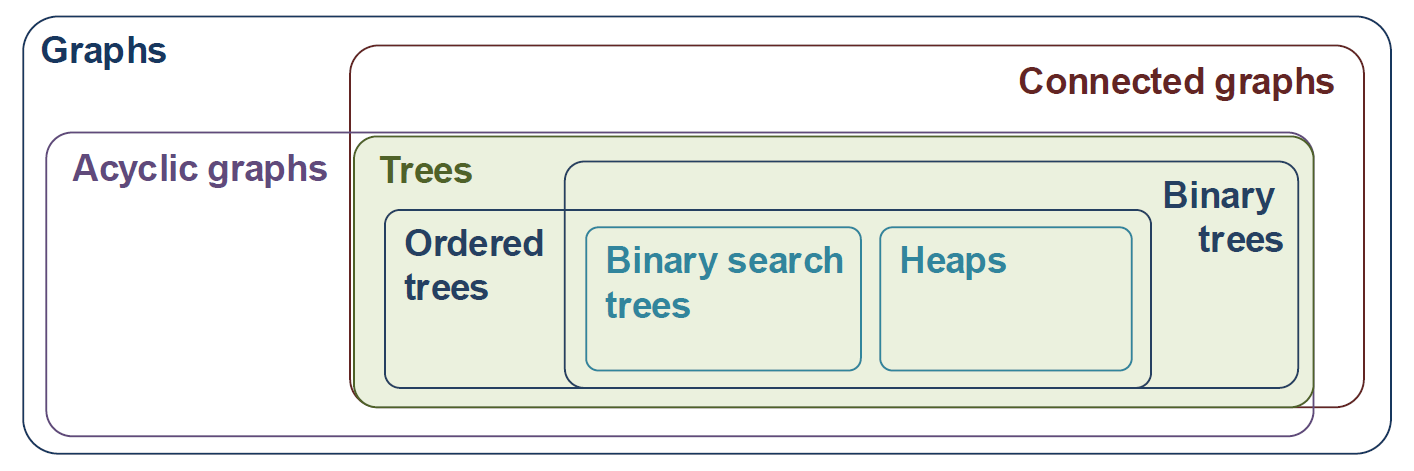
\includegraphics[width=0.85\textwidth]{img/graphs/GraphsTrees.png}\end{center}
\end{itemize}

\subsection{Representations of graphs}

A graph $G(V,E)$ with vertices $V$ and edges $E$ can be represented as a adjacency matrix (good for dense graphs) or an adjacency list (good for sparse graphs). 

\begin{center}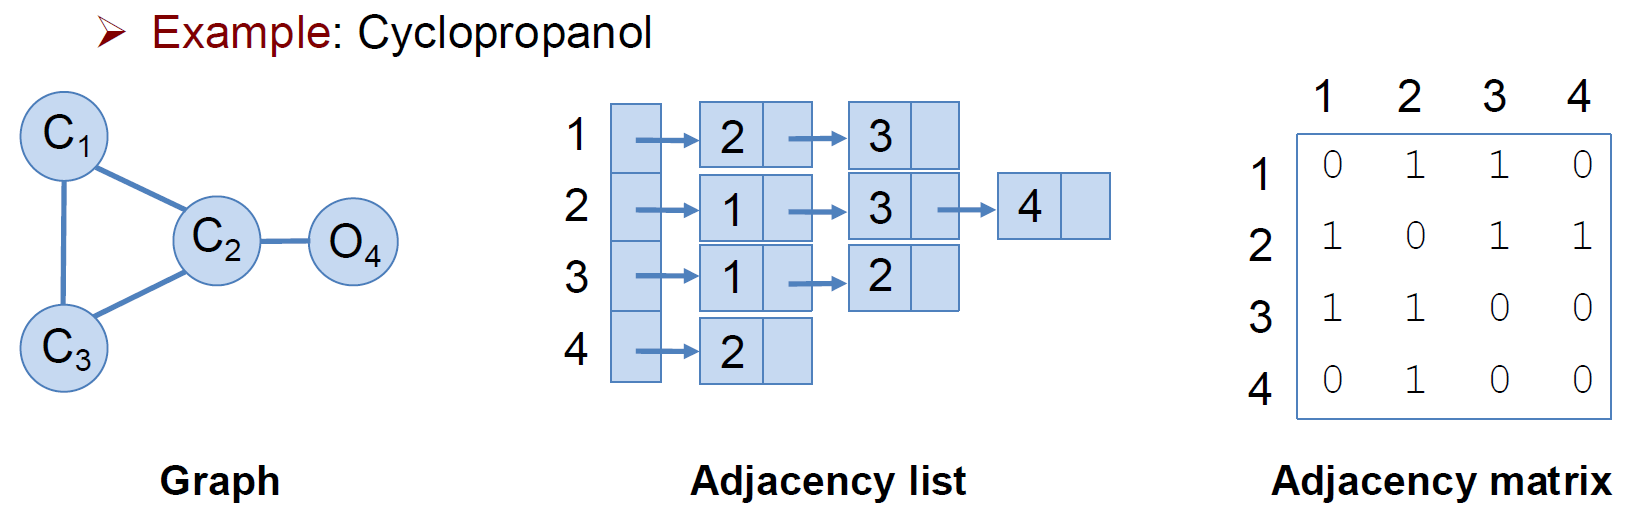
\includegraphics[width=0.85\textwidth]{img/graphs/MatrixVsList.png}\end{center}

\begin{table}[H]
    \centering
    \begin{tabular}{p{30mm} | p{50mm} | p{50mm}}
        \toprule
        \textbf{Function} & \textbf{Adjacency list} & \textbf{Adjacency matrix} \\
        \midrule
        \lstinline|size()| & Easy, size of a vector & Easy, soize of a vector \\
        \midrule
        \lstinline|isConnected()| & Difficult, search in linked list & Easy, direct access \\
        \midrule
        \lstinline|getNeighbours()| & Easy, copy of linked list & Difficult, search in row \\
        \midrule
        \lstinline|addEdge()| & Easy, append linked list & Easy, set matrix element to 1 \\
        \bottomrule
    \end{tabular}
\end{table}

\subsubsection{Adjacency list}

\lstinputlisting[language=C++]{src/graphs/graph_list.cpp}

\subsubsection{Adjacecy matrix}

\lstinputlisting[language=C++]{src/graphs/graph_matrix.cpp}

\subsection{Searching a graph}

When searching for a vertex in a graph, two different algorithms can be used: the first depth-first, the second breadth-first.

\subsubsection{Breadth-first (BF) search}

The breadth-first algorithm starts with a specific source vertex $s$, from which all vertices that can be reached from $s$ are discovered. This creates a breadth-first tree with the root $s$ and all reachable vertices.  During the algorithm, the shortest path (distance) from $s$ to $v$ is also determined for each vertex $v$. The vertices have three possible states:

\begin{itemize}
    \item \textbf{white:} undiscovered
    \item \textbf{gray:} discovered but with undiscovered neighbours
    \item \textbf{black:} discovered and all neighbours are discovered as well
\end{itemize}

All gray vertices are in a queue so that they can be processed one after the other. The running time of the algorithm is $\Theta(V+E)$

Procedure:
\begin{enumerate}
    \item First, only the given root $s$ is gray.
    \item All neighboring vertices of $s$ become gray, their distance is 1 and $s$ becomes black.
    \item All neighbors of the gray vertices become gray, their distance is 2 and the former gray vertices become black. The gray vertices in the queue are processed one after the other.
\end{enumerate}

\begin{center}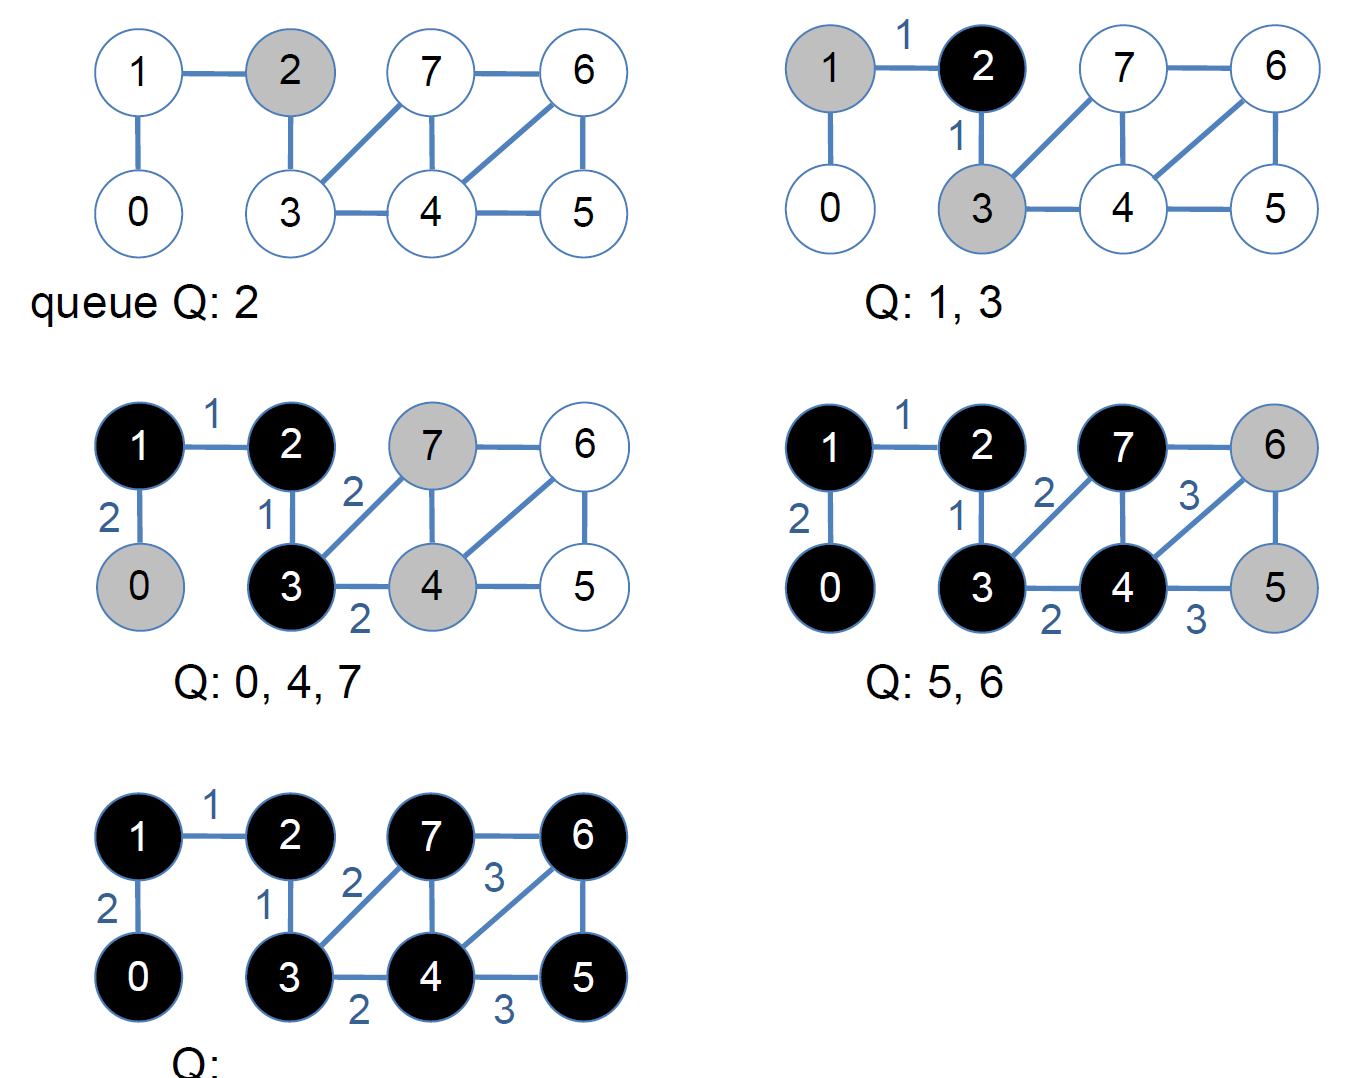
\includegraphics[width=0.85\textwidth]{img/graphs/BfSearch.png}\end{center}

\subsubsection{Depth-first (DF) search}

\subsection{Minimum spanning trees}

\subsubsection{Kruskal's algorithm}

\subsubsection{Prim's algorithm}

\subsection{Single-source shortest paths}

\subsubsection{Brute-force}

\subsubsection{Dijkstra's algorithm}

\subsection{All-pair shortest paths}

\subsubsection{Floyd-Warshall algorithm}